\documentclass{report}
\usepackage[utf8]{inputenc}
\usepackage{graphicx}
\usepackage{multirow}
\usepackage{caption}
\usepackage{subcaption}
\usepackage{amsfonts,amssymb}
\usepackage{multicol}
\usepackage{listings}
\lstset{
  basicstyle=\ttfamily,
  mathescape
}
\usepackage[utf8]{inputenc}
\usepackage[spanish]{babel}
\usepackage{lscape}
\usepackage[left=1.5cm,right=1.5cm,top=2cm,bottom=2cm]{geometry}

\begin{document}

\begin{center}
    
    \begin{tabular}{l c r}
    
\includegraphics[scale=0.15]{Imagenes/IPN.jpeg}
    & 
        \bf\fontsize{22}{0}{\selectfont{Instituto Polit\'ecnico Nacional}}

    
    & 
\includegraphics[scale=0.08]{Imagenes/escom.png} \\
     
    & \bf\fontsize{22}{0}{\selectfont{ Escuela Superior de C\'omputo}} &  \\
    \end{tabular}

	
	\vspace*{2\baselineskip}
	
	{
		\bf\fontsize{12}{0}{\selectfont{An\'alisis de Algoritmos, Sem: 2021-1, 3CV1, Pr\'actica 3, 09/11/20}}
	}
			
	\vspace*{2\baselineskip}
			 
	{
		\fontsize{23}{0}{\selectfont{Práctica 3: Complejidades temporales polinomiales y no polinomiales}}
	}
	
	\vspace*{2\baselineskip}
	
	{
		\bf\fontsize{12}{0}{\selectfont{Valle Mart\'inez Luis Eduardo, Rivero Ronquillo Omar Imanol}}
	}
	
	\vspace*{1\baselineskip}
	
	{
		\fontsize{12}{0}{\textit{lvalle212@gmail.com, imanol.rivero7@gmail.com}}
	}
	
	\vspace*{2\baselineskip}

    {
	    \fontsize{12}{0}\selectfont{
	    \textbf{Resumen:} En el actual documento se presenta el análisis, experimentación y comparación de algoritmos con complejidades del orden polinomial y aquellos  que no  son polinomiales o intratables. Para el primer algoritmo además, se muestra las implementaciones de forma iterativa y recursiva.}
	    
	    \fontsize{12}{0}\selectfont{
	    \textbf{Palabras Clave:} Complejidad, Polinomial, Java}
	
	}
\end{center}

\hfill \break
\hfill \break
\hfill \break

\section*{Introducción} 
    El objetivo principal de la informática no solamente es el de desarrollar algoritmos que resuelvan los problemas para los que fueron diseñados, sino que además, estos algoritmos deben de ser lo más eficientes que sea posible, pues de esta manera se consigue aprovechar al máximo el poder computacional que esta disponible actualmente. Existen diversos tipos de complejidades entre los que destacan aquellos de complejidad subcuadrática, y para nuestro objeto de estudio, los de complejidad de tiempo polinomial. Estos últimos son considerados por la mayoria de los científicos de la computación como los más eficientes.
\newpage

\section*{Conceptos B\'asicos}
    \subsubsection*{Polinomio}
        Dado un entero no negativo $d$, \textbf{un polinomio en $n$ de grado $d$} es una función $p(n)$ de la forma:\\
        \[ p(n) = \sum_{i=1}^{d} a_{i}n^{i}\]
        donde las constantes $a_{0},a_{1},...,a_{d}$ son los \textbf{coeficientes} del polinomio con $a_{d}\neq0$. Un polinomio es asintóticamente positivo si y sólo si $a_{d}>0$. Para un polinomio asintóticamente positivo $p(n)$ de grado $d$, tenemos $p(n) = \Theta(n^{d})$. Para cualquier constante real $a\geq0$, la función $n^{a}$ está incrementando monótonamente, y para cualquier constante real $a\leq0$, la función $n^{a}$ está decreciendo monótonamente. Se dice que una función $f(n)$ está delimitada polinómicamente si $f(n) = \mathcal{O}(n^{k})$ para alguna constante $k$.
    \subsubsection*{Complejidad Polinomial}
        Se dice que un algoritmo posee complejidad temporal polinomial si su peor caso está dado por $T(n)$ para una entrada de tamaño $n$ y tiene como límite superior un polinomio $p(n)$ para $n \geq n_{0}$.
    \subsubsection*{Sucesión de Fibonacci}
        La sucesión de Fibonacci o serie de Fibonacci, es una sucesión infinita de números definida de la siguiente forma: comienza con los números 0 y 1, a partir de éstos cada término siguiente es la suma de los dos anteriores. Teniendo como primeros elementos de la sucesión a $0, 1, 1, 2, 3, 5, 8, 13, 21, 34, 55, 89, 144, ...$.\\
    
        Se define formalmente de la siguiente forma:
        
        \begin{flushleft}
            $f_{0} = 0$\\
            $f_{1} = 1$\\
            $f_{n} = f_{n-1} + f_{n-2}$ para $n\geq2$\\
        \end{flushleft}
        
        Fue descrita por el matemático italiano Leonardo de Pisa, también conocido como Fibonacci. Este sucesión posee numerosas aplicaciones las ciencias de la computación, matemáticas y la teoría de juegos.
    \subsubsection*{Números perfectos}
        No se sabe con precisión cuando fue que se estudiaron por primera vez los números perfectos, de hecho, los primeros estudios pueden remontarse a los primeros tiempos en que los números despertaron la curiosidad de la humanidad. Es muy probable, aunque no seguro, que los egipcios se hubieran encontrado con tales números de forma natural debido a la forma en la que funcionaban sus métodos de cálculo. Pitágoras y sus seguidores estudiaron los números perfectos más por sus propiedades místicas que por sus propiedades teóricas de los números.
        
        \hfill \break

        Hoy en día, la definición habitual de los números perfectos está dada en términos de sus divisores. pero las primeras definiciones se referian a las "partes alícuotas" de un número. Una parte alícuota de un número es un cociente propio del número. Entonces las partes alícuotas de 10 son 1,2,5. Es resaltable que el 10 no es una parte alícuota de 10, ya que no es un cociente adecuado, es decir, un cociente diferente del número en sí. Un número perfecto se define como aquel que es igual a la suma de sus partes alícuotas.
        
        \hfill \break
        
        Por otro lado, tenemos la definición moderna y más conocida de los números perfectos. Un número entero positivo es perfecto, si es igual a a la suma de sus divisores menores. Por ejemplo, 8 no es un número perfecto ya que $8\neq 1 + 2 + 4$. Por otro lado, 6 sí es un número perfecto, ya que $6 = 1 + 2 + 3$. 
\newpage

\section*{Experimentación y Resultados}
    
    \hfill \break
    \hfill \break

    \subsection*{Fibonacci iterativo}
        En la situación del algoritmo de fibonacci mediante su implementación iterativa, se considera al primer elemento de la sucesión \textbf{1}, de forma que si se ingresa un valor de \textit{n} menor el valor devuelto seguira siendo 1. A partir de valores de \textit{n} mayores a 1 se mostraŕá el número que ocupa la posición \textit{n} en la sucesión infinita.
        \subsubsection*{Pseudocódigo}
            \begin{figure}[!h]
                \begin{verbatim}
                    fibonacci(n)
                        numeroSucesion = 1
                        numeroAnterior = 0
                        for i=1 to i<n do
                            numeroSucesion = numeroSucesion + numeroAnterior
                            numeroAnterior = numeroSucesion - numeroAnterior
                    return numeroSucesion
                \end{verbatim}
                \caption{Pseudocódigo de la implementación iterativa de la función Fibonacci}
            \end{figure}
            
            
        \subsubsection*{Demostración formal del orden de complejidad lineal}
            
            El algoritmo iterativo de Fibonacci mostrado en la figura [1] tendrá que el mejor y peor caso serán el mismo, por lo que el orden de complejidad es el siguiente:
            \begin{figure}[!h]
                \begin{verbatim}
                    fibonacci(n)
                        numeroSucesion = 1                                           O(1)
                        numeroAnterior = 0                                      __   O(1)
                        for i=1 to i<n do                                         |
                            numeroSucesion = numeroSucesion + numeroAnterior       > O(n)
                            numeroAnterior = numeroSucesion - numeroAnterior    __|
                    return numeroSucesion
                \end{verbatim}
                \caption{Cálculo de la complejidad del Fibonacci iterativo}
            \end{figure}
            
            En la figura [2] se aprecia que el bloque del bucle se ejecutará \textit{n-1} veces en su interior y una más cuando verifique que el valor de la variable auxiliar \textit{i} ha alcanzado el valor de \textit{n} y saldrá de su ejecución. Dado que las demás instrucciones son de complejidad constante el valor de la función será $$fibonacci(n) \in \theta (n)$$
        
        \subsubsection*{Gráficas y demostración experimental del orden de complejidad}
            Para probar de manera práctica la complejidad lineal de la función Fibonacci iterativa, se evaluarán el número de operaciones realizadas para los valores de \textit{n} que iniciarán en incremento desde el valor 1, hasta el 30 de manera incremental por unidad. A partir de este número se evaluará el número en la posición 100 incrementando los valores de 10 en 10, tal y como se muestra en la gráfica de la figura [3].
            
            \hfill \break
            
            \begin{figure}[!h]
                \centering
            	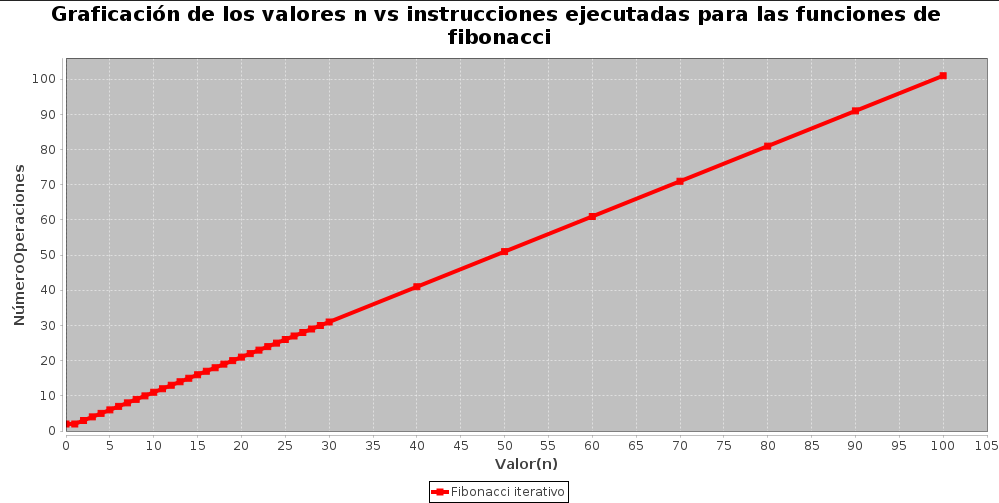
\includegraphics[width=14cm]{Imagenes/FibonacciIterativo.png}
                \caption{Gráfica que muestra en el eje de las abscisas el valor de \textit{n} y en las ordenadas el número de operaciones realizadas}
                \label{fig:my_label}
            \end{figure}
            
            Es claro el comportamiento lineal de la gráfica, por lo que se propone a partir del análisis gráfico que:
            $$fibonacci(n) \in \Theta (n)$$
    
    
    \subsection*{Fibonacci recursivo}
        \subsubsection*{Pseudocódigo}
            En lo que respecta a la implementación del algoritmo de Fibonacci mediante una solución recursiva, se identifica inicialmente el caso base. El caso base será cuando el valor del enterno \textit{n} ingresado como parámetro de la función sea igual a 1 o 0. En otro caso se realiza la suma de la llamada de 2 funciones de manera recursiva del valor de \textit{n} disminuido en la unidad y el valor de \textit{n} disminuido en 2 unidades.
            \begin{figure}[!h]
                \begin{verbatim}
                    int fibonacci(int n)
                        if n = 0 or n = 1
                            return n
                        else
                            return fibonacci(n - 1) + fibonacci(n - 2)
                \end{verbatim}
                \caption{Pseudocódigo de la implementación del algoritmo de Fibonacci de manera recursiva}
                \label{fig:my_label}
            \end{figure}
            
        \subsubsection*{Demostración formal del orden de complejidad}
            Similar a la implementación iterativa, el algoritmo descrito en la figura [4] contará con su peor y mejor caso igual, considerándose tan solo un caso promedio para un valor de \textit{n}.
            
            \newpage
            
            La ecuación de recursividad se expresa de la siguiente manera:
            \begin{figure}[!h]
                \begin{center}
                    $F(n) = 
                    \left\{
                        \begin{array}{lcc}
                            0 & si & n = 0 \\
                            1 & si & n = 1 \\
                            F(n-1) + F(n-2) & si & otro
                        \end{array}
                    \right.$
                \end{center}
                \caption{Ecuación de recursividad de la función Fibonacci}
                \label{fig:my_label}
            \end{figure}
            
            Se identifica entonces una recurrencia lineal de segundo orden y se plantea la ecuación: 
            $$F(n) - F(n-1) - F(n-2) = 0$$
            Y su ecuación característica es:
            $$\Rightarrow r^2-r-1=0$$
            Se obtienen las raíces del polinomio:
            $$r_{1,2} = \frac{1 \pm \sqrt{1 -4(-1)}}{2} = \frac{1 \pm \sqrt{5}}{2} $$
            $$r_1=\frac{1+\sqrt{5}}{2}$$
            $$r_2=\frac{1-\sqrt{5}}{2}$$
            
            Dado que el valor de las r's es diferente, se adapta el modelo de ecuación: $x(n)=\alpha r_1^n + \beta r_2^n$
            $$ F(n) = \alpha \frac{1+\sqrt{5}}{2}^n + \beta \frac{1-\sqrt{5}}{2}^n $$
            
            Ahora evaluamos nuestra función recursiva con los valores de los casos base:
            $$ 0 = F(0) = \alpha \left( \frac{1+\sqrt{5}}{2}\right)^0 + \beta\left( \frac{1-\sqrt{5}}{2}\right)^0 $$
            $$ 1 = F(1) = \alpha \left( \frac{1+\sqrt{5}}{2}\right)^1 + \beta\left( \frac{1-\sqrt{5}}{2}\right)^1 $$
            De ahí que se obtengan las siguientes ecuaciones:
            $$ 0 = \alpha + \beta $$
            $$ 1 =  \alpha \left( \frac{1+\sqrt{5}}{2}\right) + \beta\left( \frac{1-\sqrt{5}}{2}\right) $$
            $$ \Rightarrow \alpha = \frac{1}{\sqrt{5}} , \beta = -\frac{1}{\sqrt{5}} $$
            $$ \therefore F(n) = \frac{1}{\sqrt{5}}\left( \frac{1+\sqrt{5}}{2}\right)^n -\frac{1}{\sqrt{5}}\left( \frac{1-\sqrt{5}}{2}\right)^n $$
            
            Y sabemos que \textit{la relación aurea} $\phi = \frac{1+\sqrt{5}}{2}$ y $\hat{\phi} = -\frac{1}{\phi}$:
            
            $$ = \frac{1}{\sqrt{5}} \left(\phi ^n - \hat{\phi}^n \right)$$
            $$ \therefore F(n) \in \Theta (\phi ^n)$$
        
        \subsubsection*{Gráficas y propuesta experimental del orden de complejidad}
            En la siguiente figura [6] se muestra la gráfica generada por el número de operaciones realizadas de manera recursiva para encontrar el número \textit{n} de la sucesión infinita.
           
            \begin{figure}[!h]
                \centering
            	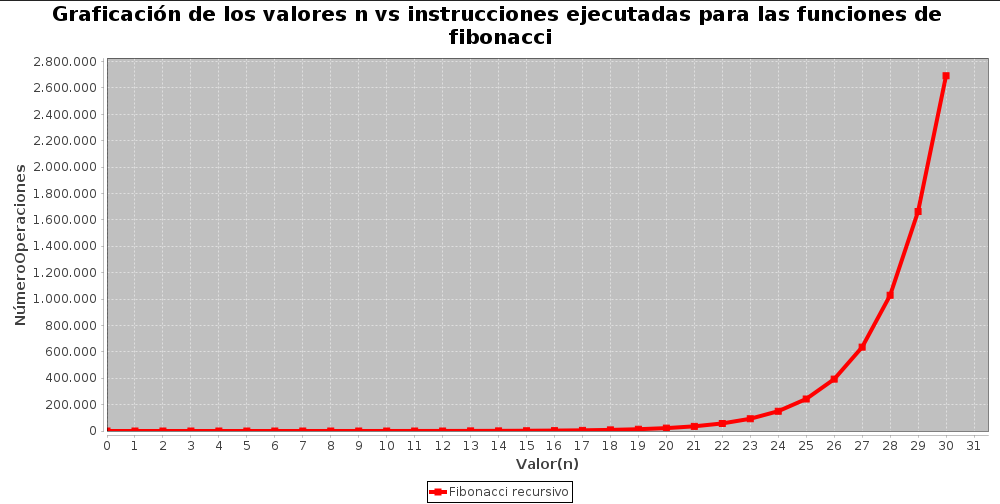
\includegraphics[width=14cm]{Imagenes/FibonacciRecursivo.png}
                \caption{Gráfica que representa en el eje de las abscisas los valores de \textit{n} y en el eje de las ordenadas el número de operaciones para la función de Fibonacci implementada recursivamente}
                \label{fig:my_label}
            \end{figure}
            
            El comportamiento mostrado por la gráfica es el de una complejidad exponencial y tomando el último punto evaluado. Con $n=30$ , el número de instrucciones ejecutadas es 2,692,537:
            $$ K^{30} = 2692537$$
            $$ K = \sqrt[30]{2692537} = 1.63809 $$
            Finalmente entonces:
            $$ fibonacci(n) \in \Theta (1.63809^n) $$
        
    \newpage
        
    \subsection*{Algoritmo Perfecto(n)}
        \subsubsection*{Pseudocódigo}
            La figura[7] muestra la implementación del algoritmo que identifica si un número de entrada \textit{n} cumple con las propiedades de un número perfecto. De ser así regresará un \textit{Verdadero}, en caso contrario un \textit{Falso}.
            El algoritmo utiliza un bucle que se ejecutará $\frac{n}{2}$ veces e ira comprobando si el valor del auxiliar puede dividir al ingreso \textit{n} como entero, de esta forma si es verdadero entonces sumará el valor del acumulador que representa la suma de los dividendos.
            
            \begin{figure}[!h]
                \begin{verbatim}
                    Perfecto(int n)
                        acumulador = 0
                        for i=0 to i<(n/2) do
                            if n % i = 0
                                acumulador++
                        if acumulador = n
                            return true
                        return false
                \end{verbatim}
                \caption{Pseudocódigo de la función que identifica si un número es considerado perfecto}
                \label{fig:my_label}
            \end{figure}    
        
        \subsubsection*{Demostración formal del orden de complejidad}
            Al igual que en los análisis anteriores de los algoritmos[4][1] , el peor y el mejor caso para el algorimo de esPerfecto(n) son el mismo.
            \begin{figure}[!h]
                \begin{lstlisting}
                    esPerfecto(int n)
                        acumulador = 0                             ___   $\mathcal{O}(1)$                   
                        for i=0 to i<=(n/2) with  i++ do              |
                            if n % i = 0                               > $\mathcal{O}(\frac{n}{2})$
                                acumulador++                       ___|
                                                            ___
                        if(acumulador = n)                     >  $\mathcal{O}(1}$ 
                            return true                     ___|
                        return false
                \end{lstlisting}
                \label{fig:my_label}
                \caption{Cálculo de complejidad por bloques de esPerfecto(n)}
            \end{figure}
            Para cualquier $n$ de entrada los pasos que tiene que ejecutar identifican una complejidad de orden lineal.
            
            $$ esPerfecto(n) \in \Theta \left( \frac{n}{2} \right) $$
            $$ \therefore esPerfecto(n) \in \Theta(n) $$
            
        \subsubsection*{Gráficas y propuesta experimental del orden de complejidad}
            En la siguiente figura [9], se muestra la gráfica generada por la relación del número de operaciones realizadas y el valor que le fue introducido al algoritmo de esPerfecto(n).\\\\
            Como podemos observar los valores introducidos van del 1 al 13, entre estos valores el único que efectivamente es un número perfecto era el 6. Es interesante resaltar el comportamiento del algoritmo para estos valores sencillos en los que a pesar de arrojar una confirmación para la entrada $n=6$, se ejecutan más operaciones comparado con el caso de $n=7$. Por lo que podriamos concluir que es indistinto el número de entrada que le demos al algoritmo, generalmente el número de instrucciones que debe de ejecutar crecera linealmente, tal como lo vimos en nuestra demostración formal.
            \\\\Finalmente, proponemos que la complejidad experimental para esPerfecto(n) está dado por $\mathcal{O}(\frac{n}{2})$. Entonces, queda demostrado nuestro cálculo formal de complejidad para este algoritmo.
            \begin{figure}[!h]
                \centering
        	    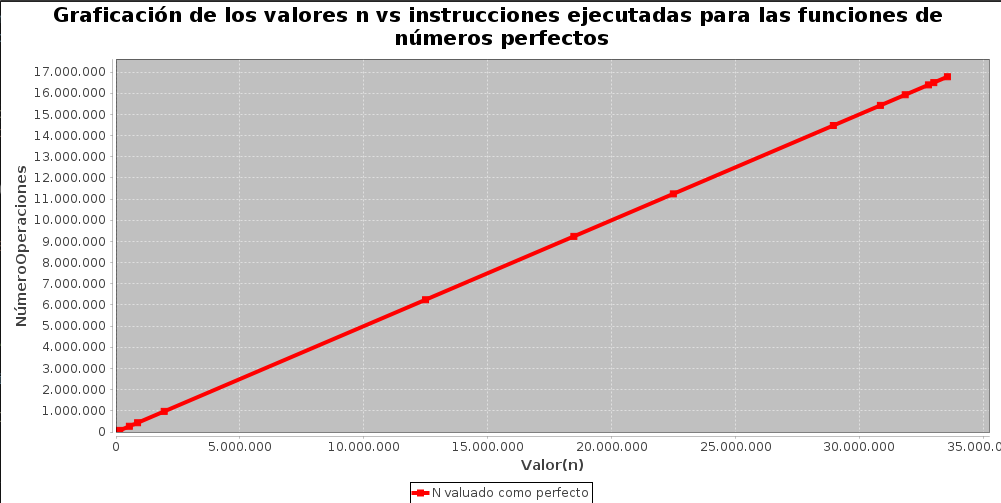
\includegraphics[width=14cm]{Imagenes/esPerfecto1.png}
                \caption{Gráfica que representa en el eje de las abscisas los valores de \textit{n} y en el eje de las ordenadas el número de operaciones para la función de esPerfecto(n) a partir de un archivo de entrada con valores de prueba.}
                \label{fig:my_label}
            \end{figure}
         \newpage
         
         A raíz de este resultado se propone la división de la evaluación del algoritmo en función de que el valor ingresado sea par o impar, permitiendonos apreciar de forma clara un comportamiento más parecido a una recta gracias a la clasificación y evitando los picos que se muestran en la figura[9].
         
         \begin{figure}[!h]
            \centering
        	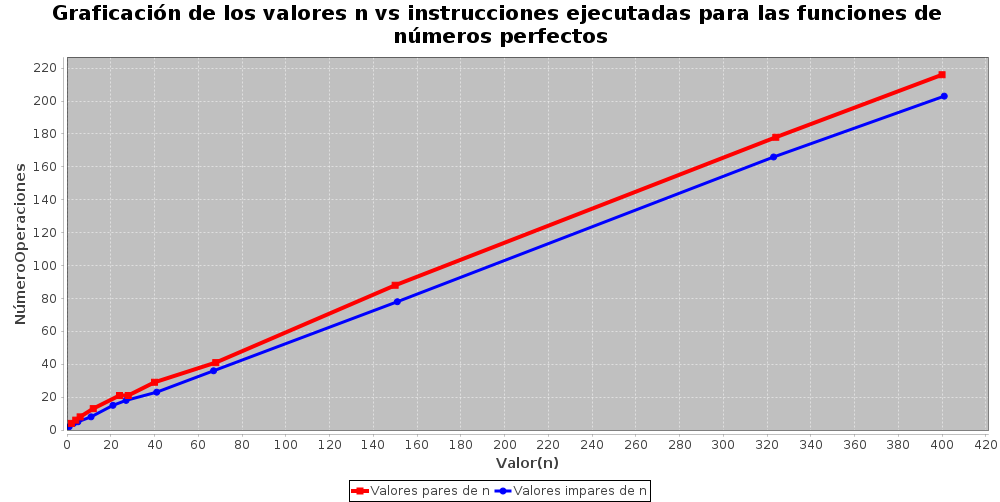
\includegraphics[width=14cm]{Imagenes/esPerfecto-PI.png}
             \caption{Gráficas generadas de la división entre impares y pares de los valores de \textit{n} en el algoritmo esPerfecto(n) }
             \label{fig:my_label}
         \end{figure}
         
         La recta que se genera por la evaluación de los números impares mantiene una pendiente muy similar a la de los valores pares, mostrando que le número de divisores y por lo tanto instrucciones realizadas, será menor para los números impares, aumentando cada vez más la diferencia entre estos.
         
        Realizadas estas consideraciones, es posible asegurar que existen las cota superior e inferior de orden lineal, Donde la superior debe acotar por arriba a la recta generada por los valores pares, y la cota inferior por debajo de la generada por los valores impares.
        $$ \therefore esPerfecto(n) \in \Theta (n) $$
         
    \subsection*{Algoritmo MostrarPerfectos(n)}
    
        \subsubsection*{Pseudocódigo}
        En la siguiente figura[9], se muestra el pseudocódigo de la función que imprime los primeros \textit{n} números perfectos. Considerando que no se ha logrado demostrar la existencia o inexistencia de un número perfecto impar, el bucle en la función ira evaluando los números pares a partir del 2 para verificar si cumple con las propiedades de un número perfecto.
        \begin{figure}[!h]
            \begin{verbatim}
                MostrarPerfectos(int n)
                    contador = 0
                    for numero = 2 to cont < n with numero+= 2 do
                        if Perfecto(numero)
                            print(acumulador)
                            contador ++
            \end{verbatim}
            \caption{Pseudocódigo de la función que permite mostrar los primeros \textit{n} números perfectos}
            \label{fig:my_label}
        \end{figure}
            
        \subsubsection*{Gráficas y propuesta experimental del orden de complejidad}
            La irregularidad de la gráfica generada nos indica un gran crecimiento del número de operaciones realizadas entre 1 número y su siguiente. Debido a la poca practicidad del cálculo de más allá de los primeros 4 números perfectos, gráficamente no es posible apreciar completamente una tendencia para relacionarla facilmente.
            \begin{figure}[!h]
                \centering
        	    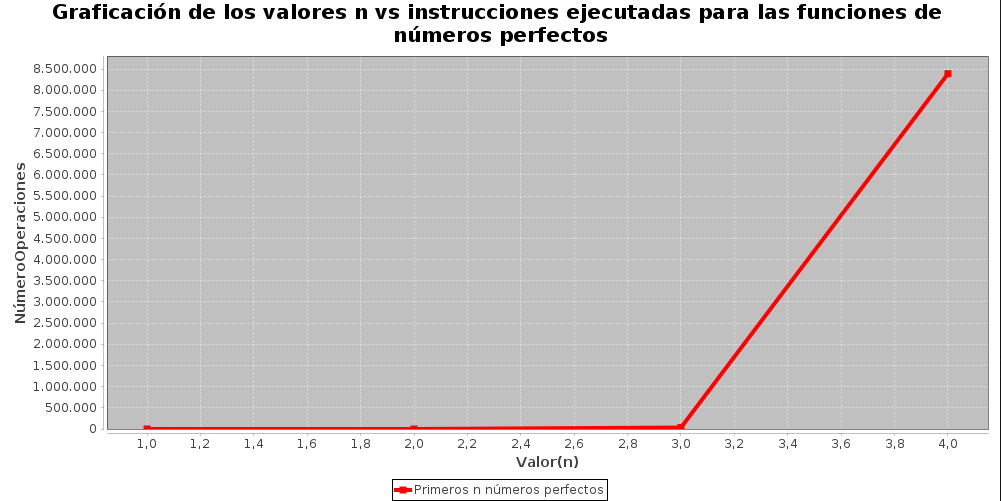
\includegraphics[width=14cm]{Imagenes/mostrarPerfectos1.png}
                \caption{Gráfica que representa en el eje de las abscisas los valores de \textit{n} y en el eje de las ordenadas el número de operaciones para la función de mostrarPerfectos(n) obteniendo los 4 primeros números perfectos.}
                \label{fig:my_label}
            \end{figure}
            
            En el algoritmo dado que se considera la imposibilidad de la existencia de números perfectos impares, el bucle se ejecutará validando números pares hasta que sea validado alguno como perfecto y el contador que define la duración del bucle aumenta la unidad, disminuyendo el número de ejecuciones restantes.
            De esta forma vamos a proponer una complejidad exponencial que va a estar multiplicando a un término lineal:
            $$ mostrarPerfectos(n) \in \Theta (2^n n) $$
        \subsubsection*{Investigación sobre el cálculo de complejidad algorítmica para MostrarPerfectos(n)}
        Una forma de encontrar números perfectos es utilizando un algoritmo 'exhaustivo'. En esta clase generalizada de algoritmos, se prueban todas las posibles opciones, para encontrar la solución deseada o la información que nos encontramos buscando. Para la tarea específica de encontrar números perfectos, implica que debemos verificar cada entero positivo, es decir, empezar a verificar desde el 1 y continuar sucesivamente verificando los números siguientes para encontrar aquellos que cumplan con la definición de número perfecto. Verificar que un número sea perfecto tiene como consecuencia recorrer un loop sobre todos los posibles divisores que la entrada pueda tener, al encontrar un divisor de la entrada debemos de mantener la suma total de estos divisores válidos y al final del proceso, comparar la suma con la entrada, en caso de que sean iguales habremos encontrado un número perfecto.\\
        
        De este modo, utilizando el enfoque exhaustivo para encontrar numeros perfectos nos encontramos con una complejidad lineal, sea cual sea la limitación que se le agregue al método esPerfecto(n).\\
        
        Se tiene conocimiento de otro enfoque para encontrar números perfectos 'turbo cargando' al método esPerfecto() utilizando los números primos. Para esto nos apoyaremos en la fórmula encontrada por Euclides.\\
        \begin{center}
            $n = 2^{p-1}(2^{p}-1)$, donde $p$ y $2^{p}-1$ son primos.\\
        \end{center}
        El algoritmo sería el siguiente:
        \begin{enumerate}
            \item Comenzamos por establecer una variable $k=1$
            \item Calculamos $m=2^{k}-1$
            \item Determinamos si m es un número primo. Para esto podemos utilizar un método simple de fuerza bruta como esPrimo(n)
            \item Si m es primo, entonces calculamos $2^{k-1}*(2^{k}-1)$. Siendo este el número perfecto asociado.
            \item Incrementamos k y repetimos el algoritmo hasta encontrar el enésimo numero perfecto requerido.
        \end{enumerate}
        
        Desde este enfoque nos arrojaría una complejidad temporal de $\mathcal{O}(logn)$. Así que 'facilmente' podremos alcanzar a encontrar el quinto número perfecto conocido, al contrario que con nuestro enfoque exhaustivo.
        
\section*{Conclusiones}
    \begin{tabular}{l l}
        \multirow{3}{*}{
\includegraphics[width=1.5cm]{Imagenes/imanol.jpg}} &  \\
        & \textbf{Rivero Ronquillo Omar Imanol}\\
        & \\
    \end{tabular}
    \vspace*{3\baselineskip}\\
    En esta ocasión, el objetivo principal de la práctica fue la comparación de algoritmos que presentan una complejidad lineal como la de fibonacci iterativo o como la de esPerfecto(n), y otros de complejidad exponencial como lo fueron fibonacci recursivo y mostrarPerfectos(n). El cambio más abrupto respecto a las prácticas pasadas fue enfrentarnos a problemas intratables según fueran los valores que trataramos de conseguir.\\
    
    Desde mi punto de vista el que más me sorprendió fue el de mostrarPerfectos() ya que para conseguir solamente el quinto valor requeria un tiempo >40 minutos de ejecución en mi computadora, cuando el número de operaciones no parecía provocar tal demostración de fuerza bruta para conseguir aquel número. Realizando una investigación más profunda sobre los números perfectos es completamente comprensible el problema que representa encontrar números cada vez más grande, algo que está consiguiendo el proyecto GIMPS desde hace ya tres décadas de arduo trabajo por los investigadores.\\
    
    En conclusión, me encantaría conocer otros problemas como estos, pues me dejan en claro el gran trabajo que representa construir algoritmos eficientes.\\\\
    \begin{tabular}{l l}
        \multirow{3}{*}{
\includegraphics[width=1.5cm]{Imagenes/lalo.jpg}}  &  \\
        & \textbf{Valle Mart\'inez Luis Eduardo} \\
        & \\
    \end{tabular}
    \vspace*{3\baselineskip}\\
    En la elaboración de la práctica se abordaron conceptos diversos relacionados con la complejidad de los logaritmos analizados. Mediante las implementaciones de los algoritmos de Fibonacci se logró comparar las complejidades de tipo polinomial mediante la generación de ecuaciónes de recurencia y ecuaciones características de polinomios.
    Para el caso de los números perfectos se plantea el concepto de algoritmos intratables, pues la ejecución de estos sobrepasa rápidamente los recursos disponibles de los equipos computacionales, aún cuando se utilice una implementación eficiente en ejecución de instrucciones implica una sobrecarga y al final desbordamiento de la memoria disponible.
    
    Es posible mejorar la complejidad de algoritmos como el de Fibonacci mediante el uso de memorización, lo que nos permite guardar los resultados ya obtenidos evitando la redundancia de cálculos resultando en una eficiencia en la ejecución de instrucciones y bajando la complejidad de su ejecución.
    
    Al igual que los algoritmos de fibonacci, es posible optimizar los algoritmos relacionados con los números perfectos, tomando algunas consideraciones, o utilizando otros principios algorítmicos como el de Euclides para disminuir el número de cálculos.
    
\newpage

\begin{thebibliography}{X}
    \bibitem{libro}Cormen, T., (2009). Introduction To Algorithms. 3rd ed. Cambridge, Mass.: MIT Press.
    \bibitem{articulo1}O'Connor, J. J., Robertson E. F. (2020, Enero). Perfect Numbers. University of St Andrews, Scotland. MathsHistory. Recuperado de https://mathshistory.st-andrews.ac.uk/HistTopics/Perfect$_$numbers/
    \bibitem{articulo2}Perfect numbers. (2020, Septiembre, 19). Standford-Edu. Stanford University, California. Recuperado de https://web.stanford.edu/class/cs106b/assignments/1-cpp/perfect
\end{thebibliography}
\end{document}

